\documentclass[12pt]{article}
\usepackage{amsmath, amssymb, amsfonts, bm, graphicx, geometry, tabularx, booktabs, float, enumitem}
\geometry{margin=1in}

\title{}
\date{}
\author{}

% Uppercase Volume with thicker, higher line
\newcommand{\vol}{\mathord{\text{\ooalign{\hidewidth $V$\hidewidth\cr\kern-0.5pt\raisebox{0.8ex}{\rule[0pt]{1em}{0.5pt}}}}}}

% Lowercase Volume with built-in shifts
\newcommand{\svol}{%
  \mathord{\text{\ooalign{%
    \hspace{0.1em}$v$\cr         % built-in horizontal shift of 'v'
    \hspace{-0.02em}\rule[0.6ex]{0.8em}{0.5pt} % built-in horizontal shift of the bar, vertical raise, length, thickness
  }}}%
}
\begin{document}

\section*{3-26E}
\vspace{-1em}
\begin{center}
    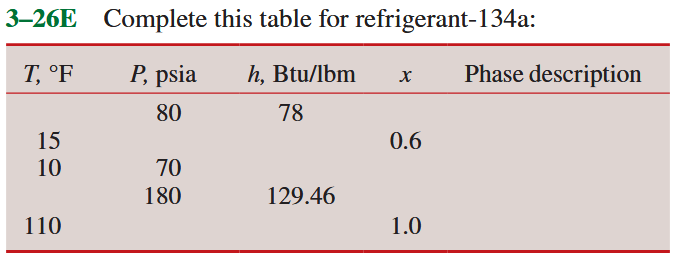
\includegraphics[width=0.6\textwidth]{3-26E.png}
\end{center}
\renewcommand{\arraystretch}{1.2}
\begin{center}
\begin{tabular}{c c c c l}
\hline
$T~(^\circ\text{F})$ & $P~(\text{psia})$ & $h~(\text{Btu/lbm})$ & $x = \frac{h-h_f}{h_{fg}}$ & Phase description \\ 
\hline
\textbf{65.89} & 80 & 78 & \textbf{0.46} & \textbf{saturated mixture} \\
15 & \textbf{29.759} & \textbf{69.92} & 0.6 & \textbf{saturated mixture} \\
10 & 70 & \textbf{$\approx$ $h_f$ = 15.308} &\textbf{--}  & \textbf{compressed liquid, $P>P_{\text{sat}}$} \\
\textbf{117.69} & 180 & 129.46 & \textbf{--} & \textbf{superheated vapor} \\
110 & \textbf{161.16 } & \textbf{117.25} & 1.0 & \textbf{saturated vapor} \\
\hline
\end{tabular}
\end{center}
For phase, compare the enthalpy to the saturated liquid and vapor enthalpies. If $h < h_f$, the phase is compressed liquid. If $h > h_{fg}$, the phase is superheated vapor. If $h_f < h < h_{fg}$, the phase is saturated mixture.\\\\
\[h_\text{avg} = h_f+x(h_{fg})\]
\section*{3-37}
\vspace{-1em}
\begin{minipage}[t]{0.6\textwidth} \vspace{0pt}
\centering
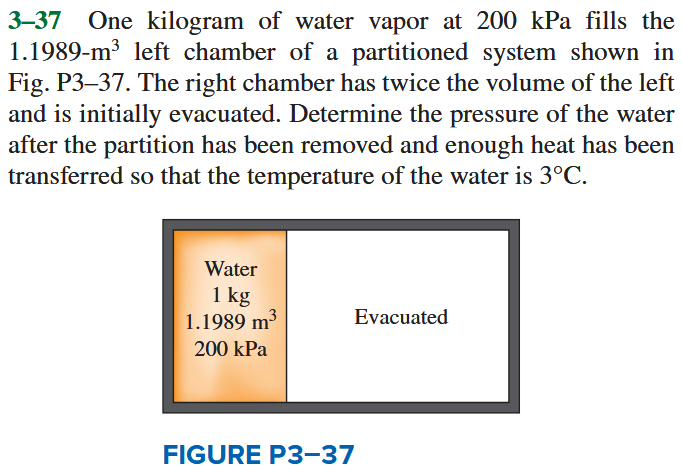
\includegraphics[width=\textwidth]{3-37.png}
\end{minipage}
\hfill
\begin{minipage}[t]{0.4\textwidth} \vspace{0pt}
Given:
\begin{itemize}
    \item mass $m=1$ kg
    \item pressure $P=200$ kPa
    \item volume $\vol=1.1989$ m$^3$
    \item water vapor
    \item Right chamber has volume 2$\vol$ and is evacuated
\end{itemize}
Find: 
\begin{itemize}
    \item Pressure of water after partition is open and it has temp $T=3^\circ$C
\end{itemize}
\end{minipage}\\\\
\textbf{State 1:} 
\[\svol_1 = \frac{\vol}{m} = \frac{1.1989}{1} = 1.1989~\text{m}^3/\text{kg}\]
\textbf{State 2:}
\[\svol_2 = \frac{3\vol}{m} = \frac{3(1.1989)}{1} = 3.5967~\text{m}^3/\text{kg}\]
Using the specific volume at state 2, it is a saturated mixture, so we can use table A-4 to find the saturation pressure (via linear interpolation):
\[P_2-P_1=m(T_2-T_1) \quad \implies P_2 - [0.8725\,\text{kPa}] = (0.0522)\left([3^\circ C] - [5^\circ C]\right)\]
\[\boxed{P_2 = P_{\text{sat @ 3}^\circ C}=0.7679\,\text{kPa}}\]
\section*{3-43}
\vspace{-1em}
\begin{minipage}[t]{0.6\textwidth} \vspace{0pt}
\centering

\includegraphics[width=\textwidth]{3-43.png}
\end{minipage}
\hfill
\begin{minipage}[t]{0.4\textwidth} \vspace{0pt}
Given:
\begin{itemize}
    \item 
\end{itemize}
Find: 
\begin{itemize}
    \item 
\end{itemize}
\end{minipage}\\\\
\section*{3-60}
\vspace{-1em}
\begin{minipage}[t]{0.6\textwidth} \vspace{0pt}
\centering

\includegraphics[width=\textwidth]{3-60.png}
\end{minipage}
\hfill
\begin{minipage}[t]{0.4\textwidth} \vspace{0pt}
Given:
\begin{itemize}
    \item 
\end{itemize}
Find: 
\begin{itemize}
    \item 
\end{itemize}
\end{minipage}\\\\
\section*{3-69}
\vspace{-1em}
\begin{minipage}[t]{0.6\textwidth} \vspace{0pt}
\centering
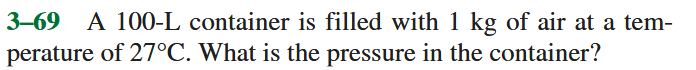
\includegraphics[width=\textwidth]{3-69.png}
\end{minipage}
\hfill
\begin{minipage}[t]{0.4\textwidth} \vspace{0pt}
Given:
\begin{itemize}
    \item 
\end{itemize}
Find: 
\begin{itemize}
    \item 
\end{itemize}
\end{minipage}\\\\
\section*{3-75}
\vspace{-1em}
\begin{minipage}[t]{0.6\textwidth} \vspace{0pt}
\centering
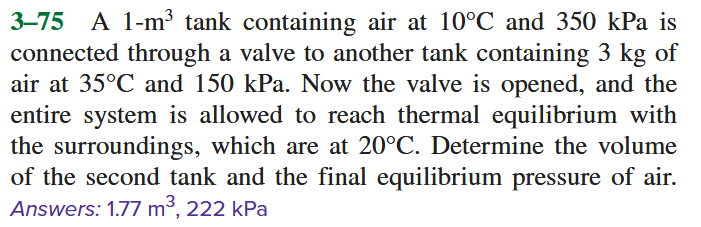
\includegraphics[width=\textwidth]{3-75.png}
\end{minipage}
\hfill
\begin{minipage}[t]{0.4\textwidth} \vspace{0pt}
Given:
\begin{itemize}
    \item 
\end{itemize}
Find: 
\begin{itemize}
    \item 
\end{itemize}
\end{minipage}\\\\
\section*{3-95E}
\vspace{-1em}
\begin{minipage}[t]{0.6\textwidth} \vspace{0pt}
\centering
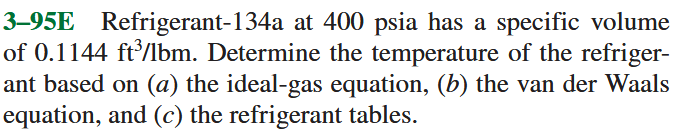
\includegraphics[width=\textwidth]{3-95E.png}
\end{minipage}
\hfill
\begin{minipage}[t]{0.4\textwidth} \vspace{0pt}
Given:
\begin{itemize}
    \item 
\end{itemize}
Find: 
\begin{itemize}
    \item 
\end{itemize}
\end{minipage}\\\\
\section*{3-136}
\vspace{-1em}
\begin{minipage}[t]{0.6\textwidth} \vspace{0pt}
\centering
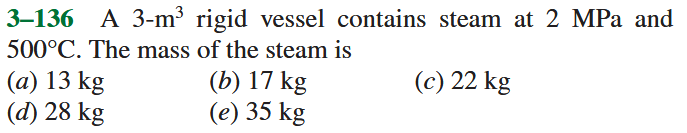
\includegraphics[width=\textwidth]{3-136.png}
\end{minipage}
\hfill
\begin{minipage}[t]{0.4\textwidth} \vspace{0pt}
Given:
\begin{itemize}
    \item 
\end{itemize}
Find: 
\begin{itemize}
    \item 
\end{itemize}
\end{minipage}\\\\

\end{document}